\documentclass{IEEEtran}
\usepackage{cite}
\usepackage{amsmath,amssymb,amsfonts}
\usepackage{algorithmic}
\usepackage{graphicx}
\usepackage{textcomp}

% Disable all paragraph indentation
\setlength{\parindent}{0pt}

\def\BibTeX{{\rm B\kern-.05em{\sc i\kern-.025em b}\kern-.08em
    T\kern-.1667em\lower.7ex\hbox{E}\kern-.125emX}}
\begin{document}
\title{Flu Shot Learning: \\Predicting H1N1 and Seasonal Flu Vaccination}
\author{Jorge Pais, José Baptista and Pedro Duartee\\ 
    \textit{up201904841@edu.fe.up.pt; up201904814@edu.fe.up.pt; up201905050@edu.fe.up.pt}}

\maketitle

\begin{abstract}
    %The model used in this study was a gradient boosting classifier, which was evaluated on separate test data provided by the NHFS using the area under the Receiver Operating Characteristic (ROC) curve as a performance metric. After necessary parameter tuning, the model was able to achieve a score of 0.8415.
\end{abstract}

\section{Introduction}
Pandemics have rarely taken center stage in the way they have recently with COVID-19 in 2020.  Vaccines are a key public health measure used to fight infectious diseases like COVID-19. They provide immunization for individuals, and enough immunization in a community can further reduce the spread of diseases through "herd immunity." 
In 2009, the H1N1 influenza virus, also known as swine flu, caused a global pandemic that was estimated to have resulted in 150,000 to 600,000 deaths worldwide. A vaccine for H1N1 became available in October of that year. In this study, a machine learning model was developed to help estimate the probability of a person receiving seasonal and H1N1 vaccines. For this, several classification methods were explored and compared between each other in order to figure out which one exhibited the best performance.

\section{Data Resources}

For the competition partaken in this project, the dataset was provided by DrivenData, and it comes from the National 2009 H1N1 Flu Survey (NHFS) which was collected through telephone interviews. The dataset consists of 36 attributes, varying from numerical with both ordinal and binary variables, and also categorical attributes. For the training data, there were 2 labels associated with each respondent, indicating whether or not each respondent had taken the H1N1 and Seasonal flu vaccines.

\subsection{Data Cleaning and Pre-processing}
The first step in the data analysis was to check if the data has any duplicate (i.e. duplicate respondent ids) and missing values, duplicates were not observed, but the dataset had many missing values in different attributes. So, the first concern was to clean the data. Since the attributes employment concern and employment occupation had the highest missing data (13470 values) we decided to drop the same along with respondent id as it was of no use. The next step involved checking of correlation  between the attributes. This was done using the \textit{Seaborn} library's correlation heatmap. It was noted that some attributes exhibited mild positive correlation, with two stand-out attributes named \texttt{doctor recc H1N1 vaccine} and \texttt{doctor recc seasonal vaccine}, which were positively correlated by 60\%.

In the next step, the missing data were handled. Two different imputation methods are implemented in this project, the first one being median imputation and the second one, the one-hot encoder. The algorithms and packages used in this work require numeric data, and not categorical data. Therefore, a unique numerical value is assigned to each category in the object columns. This method can cause problems, as the model might not recognize the data as categorical and would process it on a scale. This leads to incorrect weight assignments. To avoid this problem, one-hot encoder is used, which encodes a category in a 1-hot vector, where the position in the vector refers to each category and its size is equal to the number of categories. Simple imputer is used to fill in missing data using median method. The \textit{Pandas} library in Python identifies missing values as \texttt{NaN}. After the data is cleaned and pre-processed, graphical visualizations are generated.
\begin{center}
    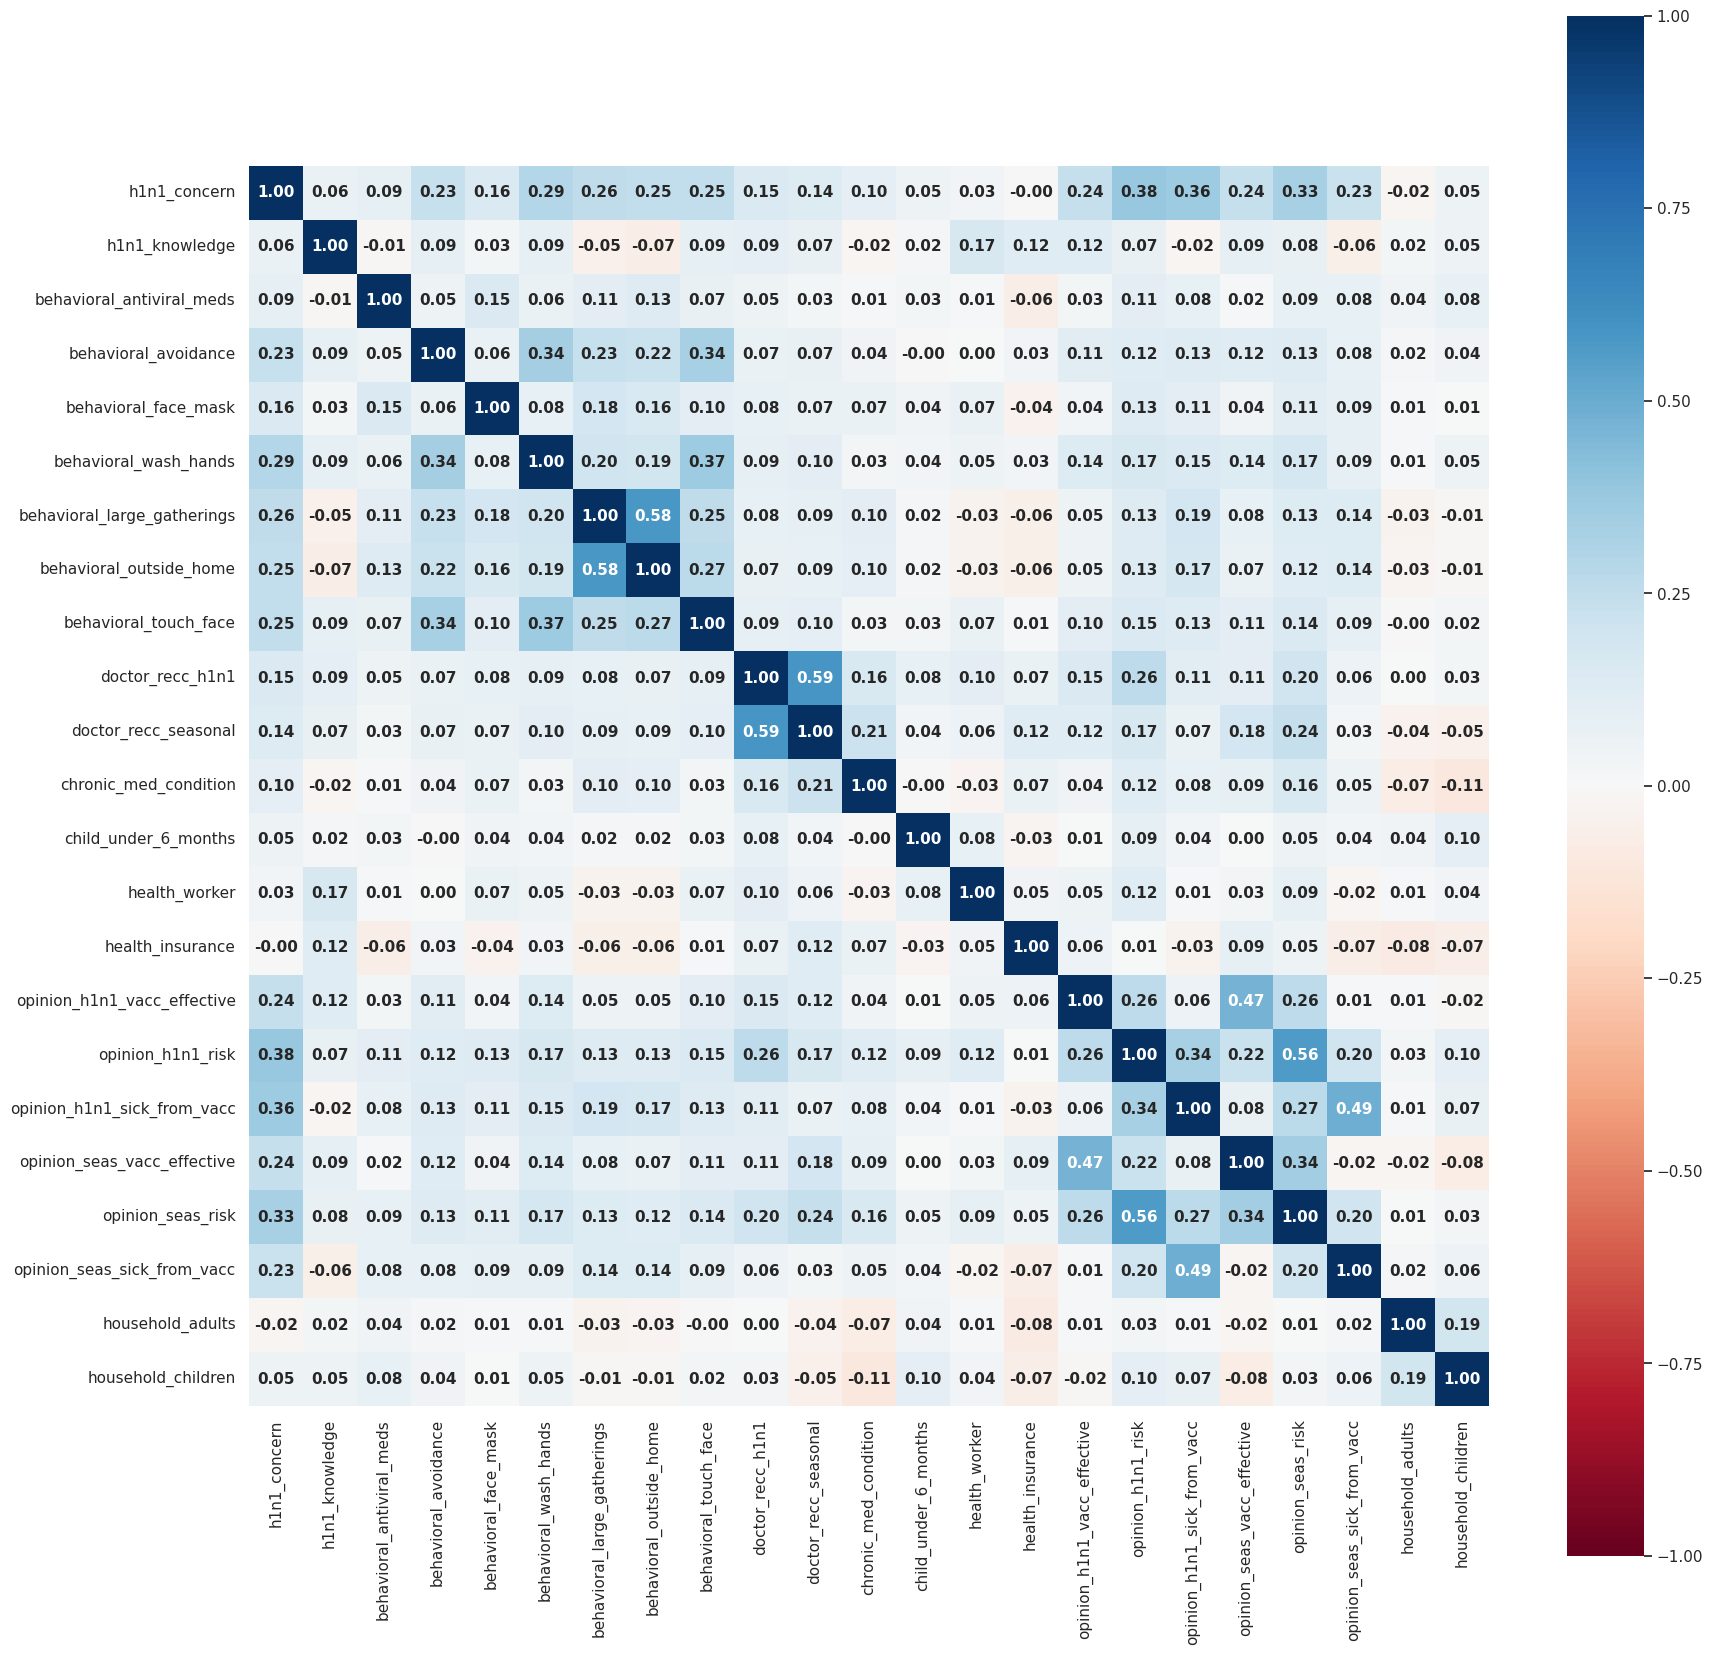
\includegraphics[width = 8cm,height=8cm]{figures/Heatmap.png}\\  
    Figure 2.1 - Feature Correlation Heatmap
\end{center}

\subsection{Class Balance}
Different attributes are plotted to check how the data is distributed. 

Approximately half of individuals have been vaccinated for the seasonal flu, while only 20\% have been vaccinated for H1N1. As for class balance, we can say that the distribution of individuals vaccinated for the seasonal flu is balanced, while the distribution of those vaccinated for H1N1 is moderately imbalanced.
\begin{center}
    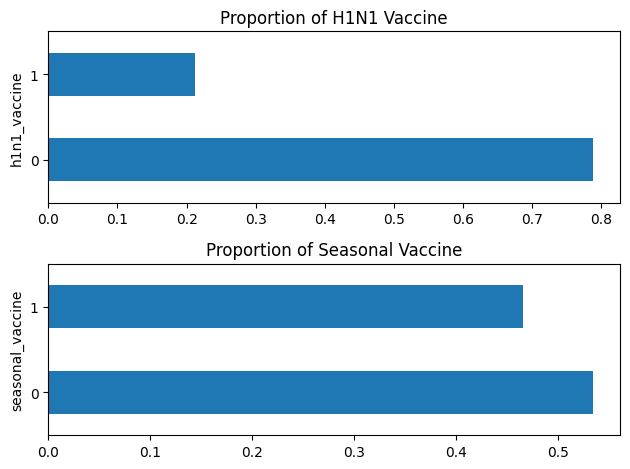
\includegraphics[width = 8cm,height=7cm]{figures/Proportion.png}\\  
    Figure 2.1 - Feature Correlation Heatmap
\end{center}
Firstly, it is observed that out of the people who received the seasonal vaccine, most of them were female. The same case was also observed with H1N1 vaccine through which one can conclude that women are more prone to get affected than men.
\begin{center}
    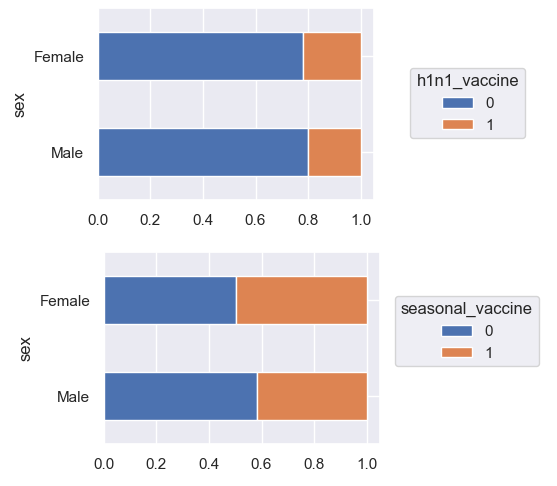
\includegraphics[width = 8cm,height=7cm]{figures/Sex.png}\\  Figure 2 - Vaccination for male and female
\end{center}

The age group has a strong correlation with the seasonal flu vaccine but not with the H1N1 flu vaccine. It seems that people act appropriately when it comes to the seasonal flu as older individuals have a higher risk of complications. However, with H1N1 flu, even though older individuals have a higher risk of complications, they are less likely to get infected. This analysis does not provide information about causality, but it seems that the risk factors are reflected in vaccination rates.
It appears that questions related to knowledge and opinions have a strong correlation with both target variables. Finally we got a  graph to conclude white people received the highest vaccination than any other race that is depicted which is more evident with the seasonal flu vaccine, but not as much with the H1N1 flu vaccine. 

\begin{center}
    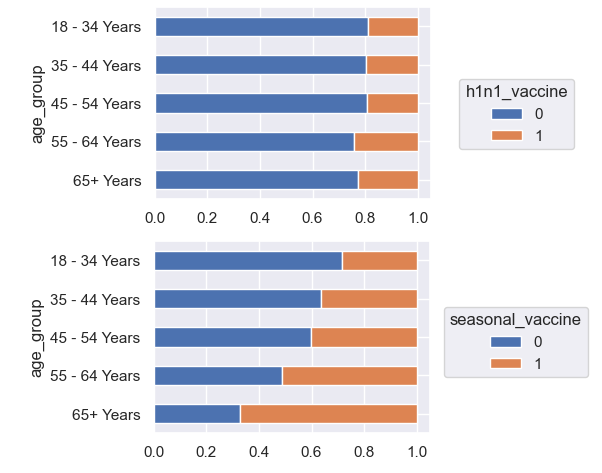
\includegraphics[width = 8cm]{figures/Age.png}\\
    Figure 2.2 - Vaccination for different age groups
\end{center}



\section{Performance Metric}
To measure the performance of the classifications performed between different classifiers, the ROC (Receiver Operating Characteristic) metric was utilized. The ROC is a type of plot used in binary classifiers, which measures the true positive rate (TPR) against the false positive rate (FPR) for different classifier thresholds. To obtain a quantitative measurement of the performance obtained, it it possible to take the area under the curve (AUC). One way of interpreting AUC is as the probability that the model ranks a random positive example more highly than a random negative example. Note that this area can be between 0 and 1, the latter characterizing a perfect classifier.
Firstly, the AUC was calculated for a \textit{Dummy Classifier}. It is a classifier model that makes predictions without trying to find patterns in the data, serving as a simple baseline to compare with other more complex classifiers. The strategy used to generate predictions was "uniform", in order to generate predictions uniformly at random. The value obtained for the AUC of the H1N1 vaccine can be seen in the graph in figure 3.1.

\begin{center}
    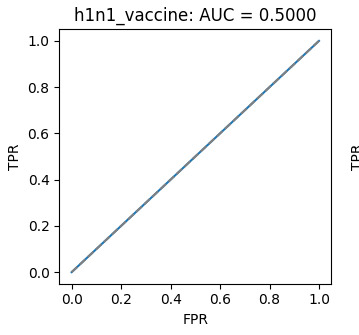
\includegraphics[width=7cm]{figures/ROC_Dummy_Classifier.png}\\
    Figure 3.1 - ROC curve for \textit{Dummy Classifier} (H1N1 vaccine)
\end{center}

After that, using the same method, the classification performance of different experimented classifiers was measured. One of the best results was obtained with the \textit{CatBoost} model, whose graph for the seasonal vaccine is represented in figure 3.2.

\begin{center}
    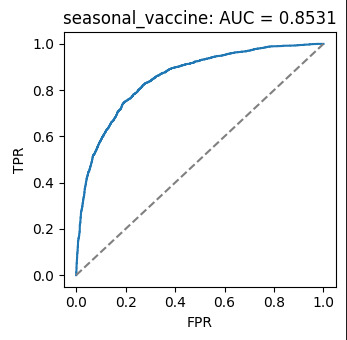
\includegraphics[width=7cm]{figures/ROC_CatBoost.png}\\
    Figure 3.2 - ROC curve for \textit{CatBoost} (seasonal vaccine)
\end{center}

\section{Methodology}
As mentioned previously, several classification models were experimented with and compared. Some of the standard classification models utilized for the purposes of this project included Logistic Regression, Multinomial Naive Bayes, K-Nearest neighbors and Decision Trees. Besides these, two gradient boosting algorithms, \textit{CatBoost} and \textit{XGBoost} were also used.
For most of the models, in order to automate the data processing and estimation steps, \textit{SKLearn} pipelines were utilized. Within the preprocessing steps, column transformations were performed separately for the numerical and categorical features. For the numerical processing, the \texttt{StandardScaler} \textit{SKLearn} class was utilized in most cases to guarantee that each column had nil mean and unit variance, followed by \texttt{SimpleImputer} to fill all missing data values utilizing each columns median value.

For categorical features, missing data was also filled using \texttt{SimpleImputer()}, but this time with the most frequent value, before being encoded utilizing an One-Hot Encoder, which separated each possible category within each feature into separate binary variables.
For the estimation, since most classifiers utilized did not support multi-label classification, the \texttt{MultiOutputClassifier()} function was utilized, which in the this case will train two separate instances of the desired estimator.

For measuring the performance of the classifiers obtained before submitting any results for the competition (only 3 daily submissions were allowed on this competition), the training set was split/folded randomly using \texttt{train\_test\_split()} to obtain a performance measurement. After this, the models were trained on the entire dataset. Figure 4.1. illustrates this entire process.

\begin{center}
    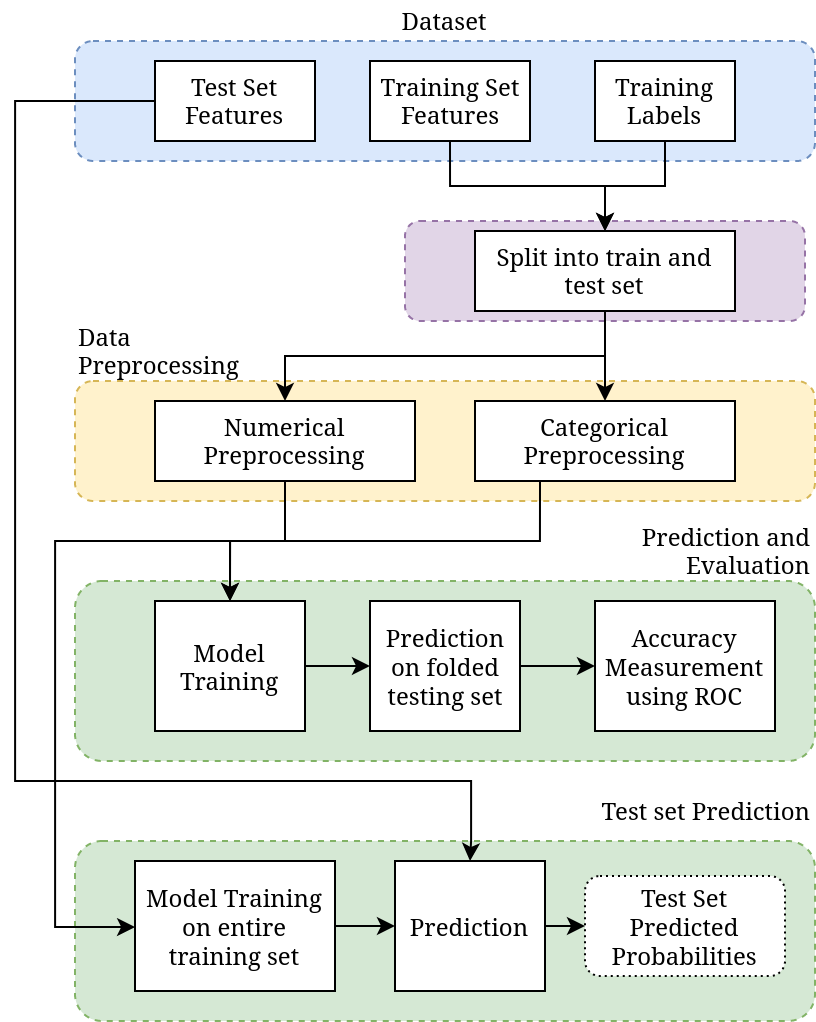
\includegraphics[width=7cm]{figures/MethodologyStructure.png}\\
    Figure 4.1 - Model Structure used
\end{center}

\subsection{Logistic Regression}
The first model to be trained was the Logistic Regression. Unlike what the name suggests, the Logistic model is a classification model rather than a regression model and is one of the most widely used techniques when it comes to solving classification problems. %\\
To utilize the Logistic Regression within our model, \textit{SKLearn} already includes an implementation of this model with the class \texttt{LogisticRegression}, which includes several tweakable parameters. To iterate and compare different parameter combinations, \textit{SKLearn} includes a simple way to automate the process with the \texttt{GridSearchCV} class. This was utilized for many of the models tested, and in the case of the Logistic Regression, it was utilized to figure out the optimum type of regularization and it's strength.

\subsection{Naive Bayes}

The Naive Bayes classification methods, work by applying Bayes' Theorem naively assuming that all the features are conditionally independent from each other. The prior and posterior can then be estimated in different ways.

\textit{SKLearn} includes several Naive Bayes based classifiers, of which the \texttt{GaussianNB} and \texttt{MultinomialNB} were utilized in this project. \texttt{GaussianNB} assumes that the likelihood of each feature given the label is a gaussian function. Meanwhile, \texttt{MultinomialNB} assumes that the data is multinomially distributed, and as such it estimates the posterior probabilities by counting how often a given value appears within each label, for each feature. 

\subsection{K-Nearest Neighbors}

The K-Nearest Neighbors is a machine learning algorithm that can be used for both regression and classification. In the case of classification, the algorithm computes the $k$ closest neighbors to the observation, and classifies the observation based on what class held the majority among those neighbors.

This method can achieve very good results depending on what value of $k$ is utilized. A larger k will generally suppress the effect of noise on the data, but makes the decision boundary less clear which might affect the ROC score. To use the model, \textit{SKLearn} includes the \texttt{KNeighborsClassifier} class, which was used in combination with \texttt{GridSearchCV} to find the value $k$ that produces the best results.

\subsection{Decision Trees}

Decision Trees are models that attempt to match the target variable by learning decisions from the training data and applying these decisions to the features of an observation's features. These models have the advantage of being conceptually easy to understand, but are quite prone to overfitting the training data.

Similarly to the previous models, the \textit{SKLearn} implementation of the decisions trees, \texttt{DecisionTreeClassifier}, was utilized.

\subsection{XGBoost}

\textit{XGBoost} (which stands for eXtreme Gradient Boosting), is a library that provides many gradient boosting algorithms. Essentially, gradient boosting gives a result based on an ensemble of many weaker learning models, as for example decision trees, combining these sequentially and having each stage correct the errors of the previous one.

This library provides many different models and several interfaces for different programming environments. For the purposes of this work, the \texttt{XGBClassifier} class was used, as it easily integrates with the \textit{SKLearn}.

\subsection{CatBoost}

The final model that was utilized in this project was \textit{CatBoost}. Similarly to XGBoost, and as the name implies, \textit{CatBoost} is also a gradient boosting library. The advantage of \textit{CatBoost} is that it natively supports categorical features without any need for encoding these. This library provides a classification model, also compatible with \textit{SKLearn}, through the class \texttt{CatBoostClassifier}.

This model was utilized in two ways, firstly by integrating it into the pipeline developed previously (in the notebook \texttt{Project\_mainModel.ipynb}, including categorical feature encoding) and in a separate preprocessing pipeline in the file \texttt{Project\_catBoostedModel.ipynb}. This was done since the first the pipeline utilized \textit{SKLearn's} ColumnTransformers, which made it challenging to specify what columns were categorical in \textit{CatBoost}.

\section{Results}



\section{Conclusion}

\vfill
\pagebreak

\section{Reference Examples}

\begin{itemize}

\item \emph{Basic format for books:}\\
J. K. Author, ``Title of chapter in the book,'' in \emph{Title of His Published Book, x}th ed. City of Publisher, (only U.S. State), Country: Abbrev. of Publisher, year, ch. $x$, sec. $x$, pp. \emph{xxx--xxx.}\\
See \cite{b1,b2}.

\item \emph{Basic format for periodicals:}\\
J. K. Author, ``Name of brief,'' \emph{Abbrev. Title of Periodical}, vol. \emph{x, no}. $x, $pp\emph{. xxx--xxx, }Abbrev. Month, year, DOI. 10.1109.\emph{XXX}.123456.\\
See \cite{b3}--\cite{b5}.

\item \emph{Basic format for reports:}\\
J. K. Author, ``Title of report,'' Abbrev. Name of Co., City of Co., Abbrev. State, Country, Rep. \emph{xxx}, year.\\
See \cite{b6,b7}.

\item \emph{Basic format for handbooks:}\\
\emph{Name of Manual/Handbook, x} ed., Abbrev. Name of Co., City of Co., Abbrev. State, Country, year, pp. \emph{xxx--xxx.}\\
See \cite{b8,b9}.

\item \emph{Basic format for books (when available online):}\\
J. K. Author, ``Title of chapter in the book,'' in \emph{Title of
Published Book}, $x$th ed. City of Publisher, State, Country: Abbrev.
of Publisher, year, ch. $x$, sec. $x$, pp. \emph{xxx--xxx}. [Online].
Available: \underline{http://www.web.com}\\
See \cite{b10}--\cite{b13}.

\item \emph{Basic format for journals (when available online):}\\
J. K. Author, ``Name of brief,'' \emph{Abbrev. Title of Periodical}, vol. $x$, no. $x$, pp. \emph{xxx--xxx}, Abbrev. Month, year. Accessed on: Month, Day, year, DOI: 10.1109.\emph{XXX}.123456, [Online].\\
See \cite{b14}--\cite{b16}.

\item \emph{Basic format for briefs presented at conferences (when available online): }\\
J.K. Author. (year, month). Title. presented at abbrev. conference title. [Type of Medium]. Available: site/path/file\\
See \cite{b17}.

\item \emph{Basic format for reports and handbooks (when available online):}\\
J. K. Author. ``Title of report,'' Company. City, State, Country. Rep. no., (optional: vol./issue), Date. [Online] Available: site/path/file\\
See \cite{b18,b19}.

\item \emph{Basic format for computer programs and electronic documents (when available online): }\\
Legislative body. Number of Congress, Session. (year, month day). \emph{Number of bill or resolution}, \emph{Title}. [Type of medium]. Available: site/path/file\\
\textbf{\emph{NOTE: }ISO recommends that capitalization follow the accepted practice for the language or script in which the information is given.}\\
See \cite{b20}.

\item \emph{Basic format for patents (when available online):}\\
Name of the invention, by inventor's name. (year, month day). Patent Number [Type of medium]. Available: site/path/file\\
See \cite{b21}.

\item \emph{Basic format}\emph{for conference proceedings (published):}\\
J. K. Author, ``Title of brief,'' in \emph{Abbreviated Name of Conf.}, City of Conf., Abbrev. State (if given), Country, year, pp. \emph{xxxxxx.}\\
See \cite{b22}.

\item \emph{Example for briefs presented at conferences (unpublished):}\\
See \cite{b23}.

\item \emph{Basic format for patents}$:$\\
J. K. Author, ``Title of patent,'' U.S. Patent \emph{x xxx xxx}, Abbrev. Month, day, year.\\
See \cite{b24}.

\item \emph{Basic format for theses (M.S.) and dissertations (Ph.D.):}
\begin{enumerate}
\item J. K. Author, ``Title of thesis,'' M.S. thesis, Abbrev. Dept., Abbrev. Univ., City of Univ., Abbrev. State, year.
\item J. K. Author, ``Title of dissertation,'' Ph.D. dissertation, Abbrev. Dept., Abbrev. Univ., City of Univ., Abbrev. State, year.
\end{enumerate}
See \cite{b25,b26}.

\item \emph{Basic format for the most common types of unpublished references:}
\begin{enumerate}
\item J. K. Author, private communication, Abbrev. Month, year.
\item J. K. Author, ``Title of brief,'' unpublished.
\item J. K. Author, ``Title of brief,'' to be published.
\end{enumerate}
See \cite{b27}--\cite{b29}.

\item \emph{Basic formats for standards:}
\begin{enumerate}
\item \emph{Title of Standard}, Standard number, date.
\item \emph{Title of Standard}, Standard number, Corporate author, location, date.
\end{enumerate}
See \cite{b30,b31}.

\item \emph{Article number in~reference examples:}\\
See \cite{b32,b33}.

\item \emph{Example when using et al.:}\\
See \cite{b34}.

\end{itemize}

\begin{thebibliography}{00}

\bibitem{b1} G. O. Young, ``Synthetic structure of industrial plastics,'' in \emph{Plastics,} 2\textsuperscript{nd} ed., vol. 3, J. Peters, Ed. New York, NY, USA: McGraw-Hill, 1964, pp. 15--64.

\bibitem{b2} W.-K. Chen, \emph{Linear Networks and Systems.} Belmont, CA, USA: Wadsworth, 1993, pp. 123--135.

\bibitem{b3} J. U. Duncombe, ``Infrared navigation---Part I: An assessment of feasibility,'' \emph{IEEE Trans. Electron Devices}, vol. ED-11, no. 1, pp. 34--39, Jan. 1959, 10.1109/TED.2016.2628402.

\bibitem{b4} E. P. Wigner, ``Theory of traveling-wave optical laser,'' \emph{Phys. Rev}., vol. 134, pp. A635--A646, Dec. 1965.

\bibitem{b5} E. H. Miller, ``A note on reflector arrays,'' \emph{IEEE Trans. Antennas Propagat}., to be published.

\bibitem{b6} E. E. Reber, R. L. Michell, and C. J. Carter, ``Oxygen absorption in the earth's atmosphere,'' Aerospace Corp., Los Angeles, CA, USA, Tech. Rep. TR-0200 (4230-46)-3, Nov. 1988.

\bibitem{b7} J. H. Davis and J. R. Cogdell, ``Calibration program for the 16-foot antenna,'' Elect. Eng. Res. Lab., Univ. Texas, Austin, TX, USA, Tech. Memo. NGL-006-69-3, Nov. 15, 1987.

\bibitem{b8} \emph{Transmission Systems for Communications}, 3\textsuperscript{rd} ed., Western Electric Co., Winston-Salem, NC, USA, 1985, pp. 44--60.

\bibitem{b9} \emph{Motorola Semiconductor Data Manual}, Motorola Semiconductor Products Inc., Phoenix, AZ, USA, 1989.

\bibitem{b10} G. O. Young, ``Synthetic structure of industrial
plastics,'' in Plastics, vol. 3, Polymers of Hexadromicon, J. Peters,
Ed., 2\textsuperscript{nd} ed. New York, NY, USA: McGraw-Hill, 1964, pp. 15-64.
[Online]. Available:
\underline{http://www.bookref.com}.

\bibitem{b11} \emph{The Founders' Constitution}, Philip B. Kurland
and Ralph Lerner, eds., Chicago, IL, USA: Univ. Chicago Press, 1987.
[Online]. Available: \underline{http://press-pubs.uchicago.edu/founders/}

\bibitem{b12} The Terahertz Wave eBook. ZOmega Terahertz Corp., 2014.
[Online]. Available:
\underline{http://dl.z-thz.com/eBook/zomega\_ebook\_pdf\_1206\_sr.pdf}. Accessed on: May 19, 2014.

\bibitem{b13} Philip B. Kurland and Ralph Lerner, eds., \emph{The
Founders' Constitution.} Chicago, IL, USA: Univ. of Chicago Press,
1987, Accessed on: Feb. 28, 2010, [Online] Available:
\underline{http://press-pubs.uchicago.edu/founders/}

\bibitem{b14} J. S. Turner, ``New directions in communications,'' \emph{IEEE J. Sel. Areas Commun}., vol. 13, no. 1, pp. 11-23, Jan. 1995.

\bibitem{b15} W. P. Risk, G. S. Kino, and H. J. Shaw, ``Fiber-optic frequency shifter using a surface acoustic wave incident at an oblique angle,'' \emph{Opt. Lett.}, vol. 11, no. 2, pp. 115--117, Feb. 1986.

\bibitem{b16} P. Kopyt \emph{et al., ``}Electric properties of graphene-based conductive layers from DC up to terahertz range,'' \emph{IEEE THz Sci. Technol.,} to be published. DOI: 10.1109/TTHZ.2016.2544142.

\bibitem{b17} PROCESS Corporation, Boston, MA, USA. Intranets:
Internet technologies deployed behind the firewall for corporate
productivity. Presented at INET96 Annual Meeting. [Online].
Available: \underline{http://home.process.com/Intranets/wp2.htp}

\bibitem{b18} R. J. Hijmans and J. van Etten, ``Raster: Geographic analysis and modeling with raster data,'' R Package Version 2.0-12, Jan. 12, 2012. [Online]. Available: \underline {http://CRAN.R-project.org/package=raster} 

\bibitem{b19} Teralyzer. Lytera UG, Kirchhain, Germany [Online].
Available:
\underline{http://www.lytera.de/Terahertz\_THz\_Spectroscopy.php?id=home}, Accessed on: Jun. 5, 2014

\bibitem{b20} U.S. House. 102\textsuperscript{nd} Congress, 1\textsuperscript{st} Session. (1991, Jan. 11). \emph{H. Con. Res. 1, Sense of the Congress on Approval of}  \emph{Military Action}. [Online]. Available: LEXIS Library: GENFED File: BILLS

\bibitem{b21} Musical toothbrush with mirror, by L.M.R. Brooks. (1992, May 19). Patent D 326 189 [Online]. Available: NEXIS Library: LEXPAT File: DES

\bibitem{b22} D. B. Payne and J. R. Stern, ``Wavelength-switched pas- sively coupled single-mode optical network,'' in \emph{Proc. IOOC-ECOC,} Boston, MA, USA, 1985, pp. 585--590.

\bibitem{b23} D. Ebehard and E. Voges, ``Digital single sideband detection for interferometric sensors,'' presented at the \emph{2\textsuperscript{nd} Int. Conf. Optical Fiber Sensors,} Stuttgart, Germany, Jan. 2-5, 1984.

\bibitem{b24} G. Brandli and M. Dick, ``Alternating current fed power supply,'' U.S. Patent 4 084 217, Nov. 4, 1978.

\bibitem{b25} J. O. Williams, ``Narrow-band analyzer,'' Ph.D. dissertation, Dept. Elect. Eng., Harvard Univ., Cambridge, MA, USA, 1993.

\bibitem{b26} N. Kawasaki, ``Parametric study of thermal and chemical nonequilibrium nozzle flow,'' M.S. thesis, Dept. Electron. Eng., Osaka Univ., Osaka, Japan, 1993.

\bibitem{b27} A. Harrison, private communication, May 1995.

\bibitem{b28} B. Smith, ``An approach to graphs of linear forms,'' unpublished.

\bibitem{b29} A. Brahms, ``Representation error for real numbers in binary computer arithmetic,'' IEEE Computer Group Repository, Brief R-67-85.

\bibitem{b30} IEEE Criteria for Class IE Electric Systems, IEEE Standard 308, 1969.

\bibitem{b31} Letter Symbols for Quantities, ANSI Standard Y10.5-1968.

\bibitem{b32} R. Fardel, M. Nagel, F. Nuesch, T. Lippert, and A. Wokaun, ``Fabrication of organic light emitting diode pixels by laser-assisted forward transfer,'' \emph{Appl. Phys. Lett.}, vol. 91, no. 6, Aug. 2007, Art. no. 061103.~

\bibitem{b33} J. Zhang and N. Tansu, ``Optical gain and laser characteristics of InGaN quantum wells on ternary InGaN substrates,'' \emph{IEEE Photon. J.}, vol. 5, no. 2, Apr. 2013, Art. no. 2600111

\bibitem{b34} S. Azodolmolky~\emph{et al.}, Experimental demonstration of an impairment aware network planning and operation tool for transparent/translucent optical networks,''~\emph{J. Lightw. Technol.}, vol. 29, no. 4, pp. 439--448, Sep. 2011.

\end{thebibliography}

\end{document}
